\subsection{Kasseapperat}
I det følgende afsnit kan der læses om integrationstest for \gls{KA}.\\

\textbf{Introduktion}\\
Der er lavet integrationstests der tager udgangspunkt i vejen fra henholdsvis ShoppingList og ProductCategoryList, og ned til Connection, for at sikre at kommunikationen med \gls{CS} fungere.\\

\textbf{Testdetaljer}\\
Testene er foretaget ved hjælp af NUnit og NSubstitute. Funktionaliteten i BLL klasserme er testet med modeller \gls{SL}. For at finde ud af, hvilke klasser der skulle testes sammen er der udarbejdet et dependency tree, som kan ses på figur \ref{fig:KA-dependencies}\\

\textbf{Beskrivelse af integrationstest}\\
Som det kan ses er det et forholdsvist simpelt dependency tree, hvilket også afspejles i at der er \textit{7} integrationstests. Dette skyldes desuden at der er forholdsvis få funktionens kald ned gennem disse lag.\\
... %Grunden til at der ikke er testet fra højere lag er...

\textbf{Dependency tree}
\begin{figure}[H]
	\centering
	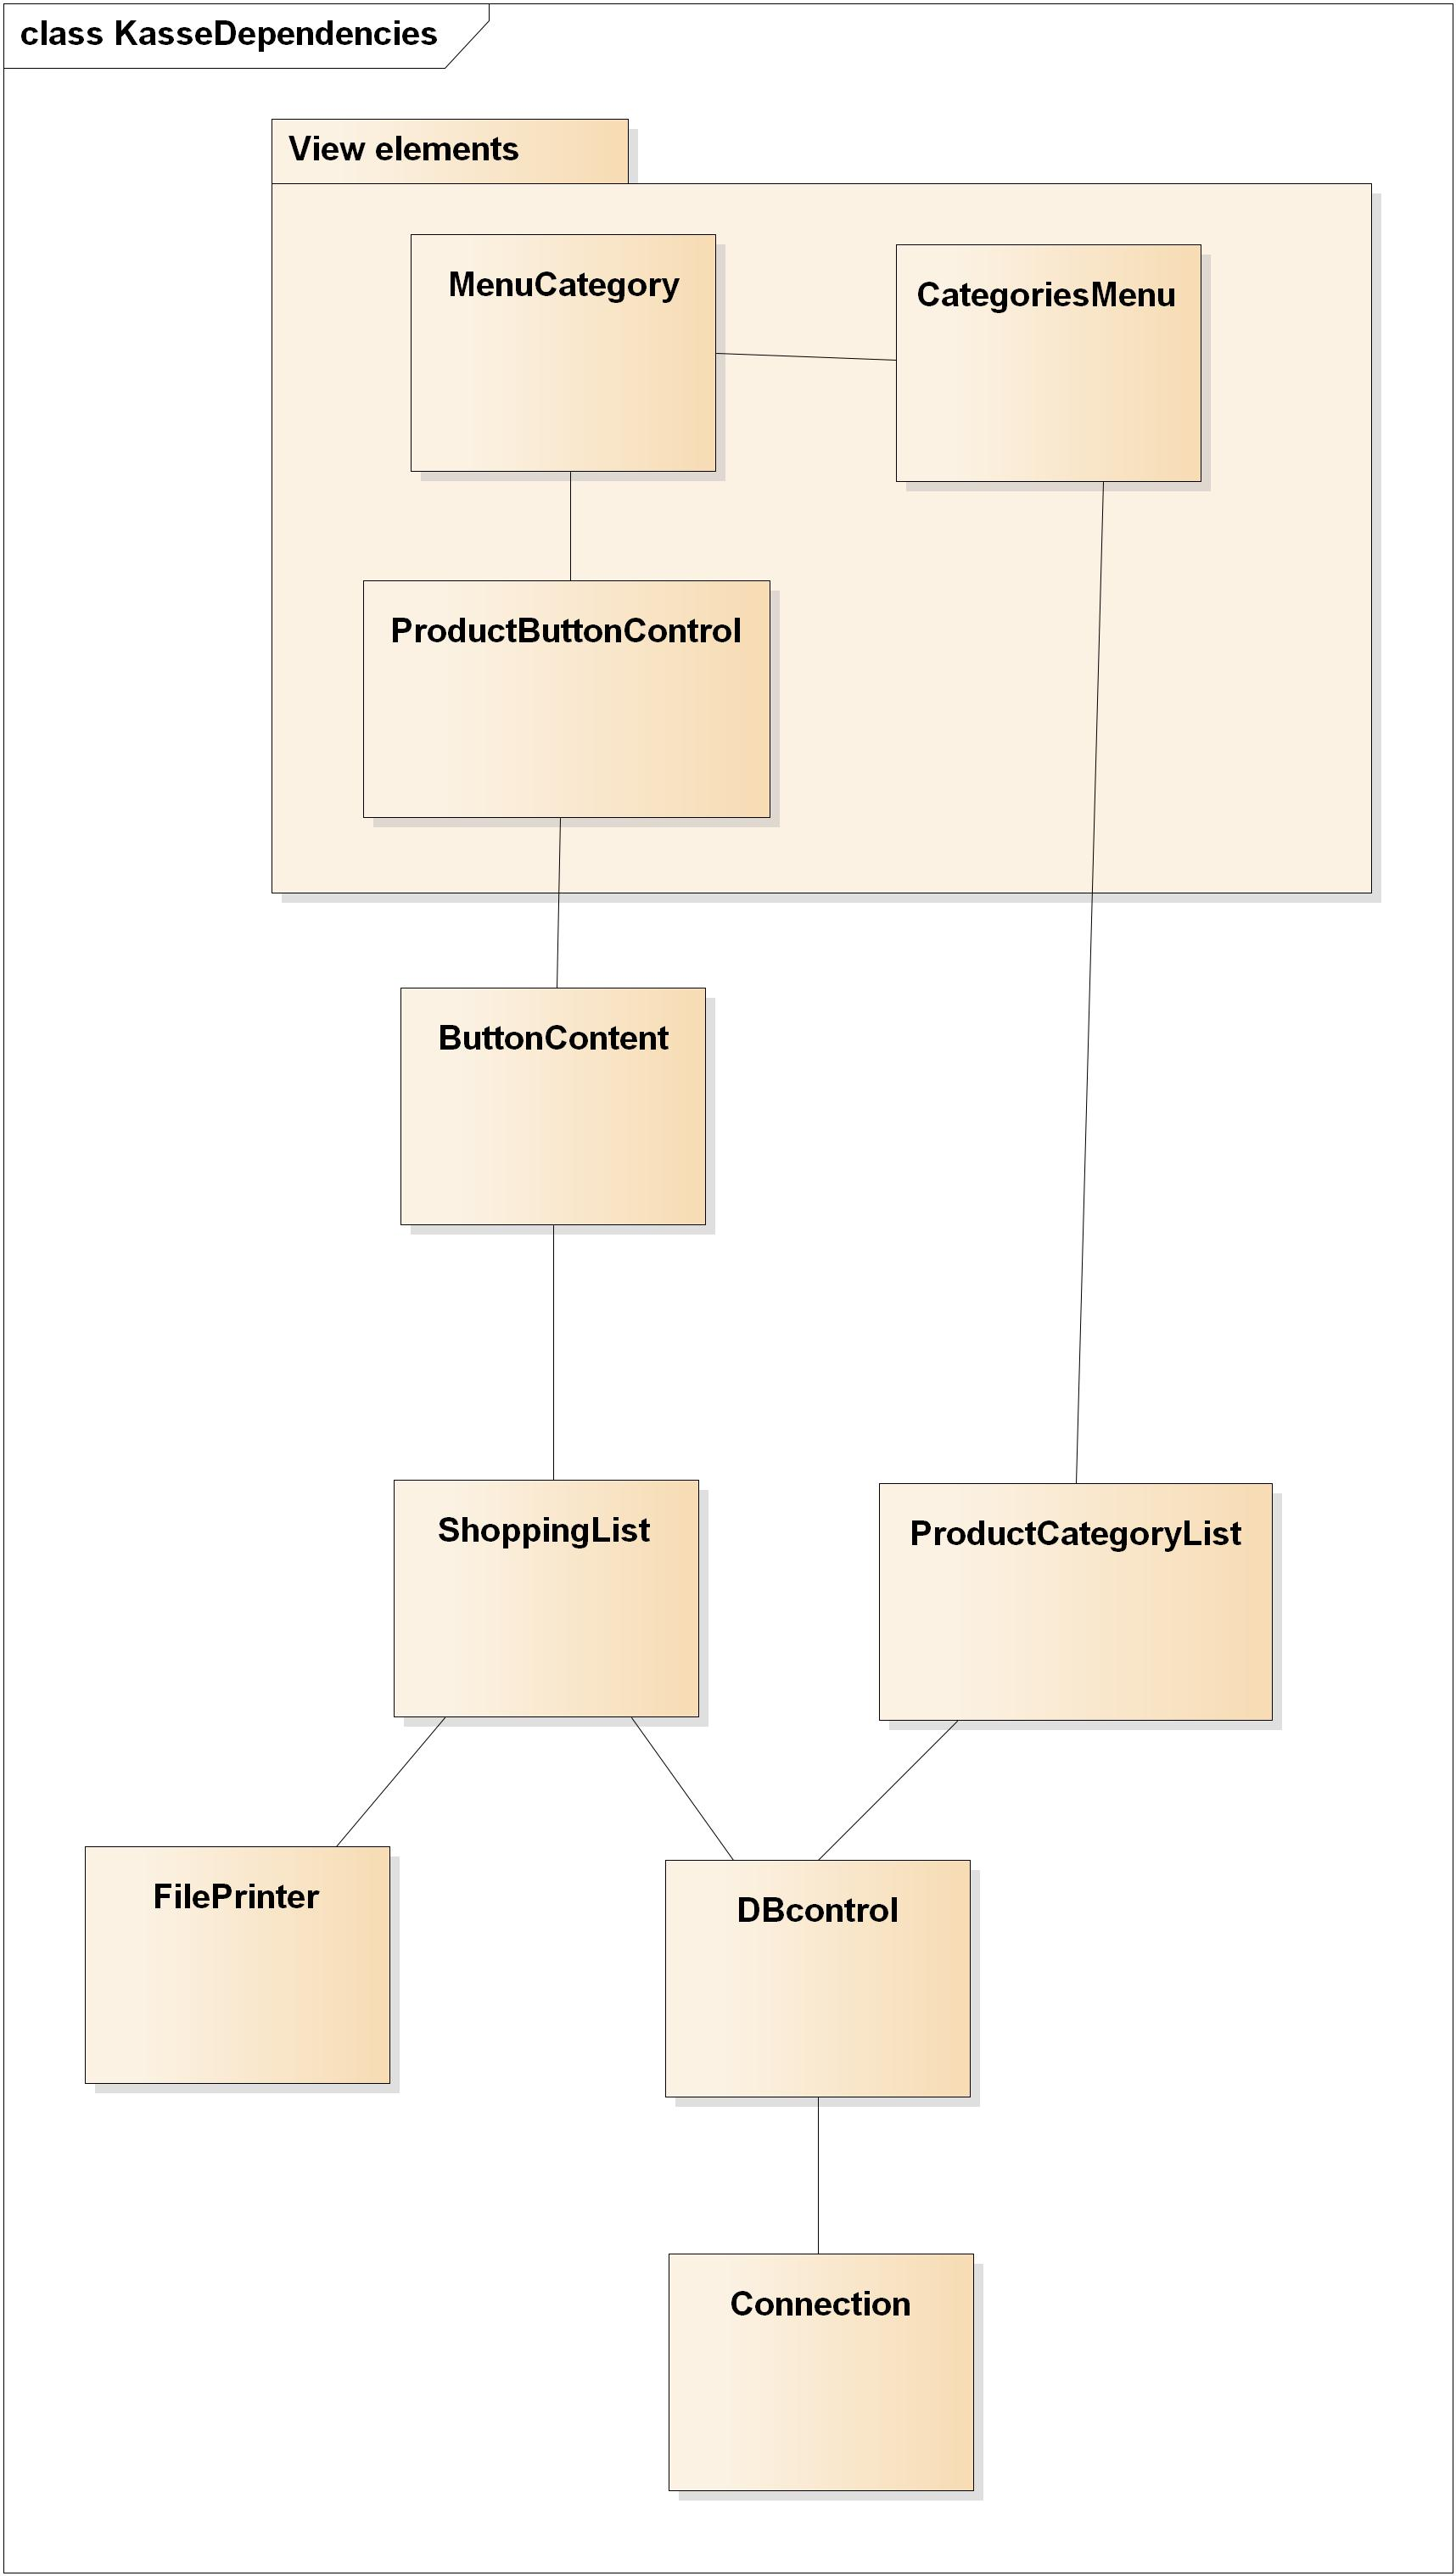
\includegraphics[width=0.7\textwidth]{Test/Integrationstest/Images/KasseDependencies}
	\caption{Dependency tree for \gls{KA}}
	\label{fig:KA-dependencies}
\end{figure}
